\chapter{Introduction}\label{ch:introduction}

\section{Background}
The respiratory rate is an important measure of a person's health and diagnosis of illnesses, defined as the number of completed breath cycles taken per minute. \cite{associationUnderstandingVitalSigns}\cite{fanHighAccuracyUltraLow2022} While respiratory rates can be affected by non-disease related factors such as exercise, emotion and elevation, in this study we are interested in Apnoea. Apnoea (commonly known as sleep apnea) is an increasingly common disorder characterised by repeated airway collapses during sleep, which can lead to oxygen desaturation and disrupted sleep. 
\cite{jordanAdultObstructiveSleep2014a} However, the measurement of respiratory rates directly can be an invasive , expensive and at times an inaccurate process. 
This has led to the underdiagnosis of Apnoea, as the diagnosis of Apnoea requires respiratory measurements. 
\nl
This has motivated research into deriving respiration from Electrocardiograms (ECGs), as these measurements are low-cost and non-invasive \cite{fanHighAccuracyUltraLow2022}. \nl
In this study, we first determine how to visualise respiratory data stored in WFDB format. Then, we will investigating a method of deriving respitatory rates through ECGs via 4th order central moments. We then compare to known datasets, and if the results are promising, then we will explore the usage of machine learning to develop a possible pipeline to diganose regions of apnoea based on ECGs.

\section{Electrocardiograms}
Electrocardiograms (ECGs) are measurements of your heart's electrical activity over time. Each beating of the heart produces a distinct pattern consisting of the P-wave, the QRS complex and the T-wave. The most relevant is the QRS complex, distinguished by the tall R-peak. \nl
A healthy person's heart rate increases and decreases slightly when breathing in and out, respectively, in a process known as Respiratory Sinus Arrythmia. These natural variations are the basis in which we can obtain information about respiration based on ECGs. If accurate information about breathing rates could be extracted, it offers a low-cost and cheap alternative to direct respiratory measurements, a process which is significantly more invasive and expensive.

\section{Reading WFDB files}
ECG readings are typically stored in the WFDB format, where a single record consists of multiple files:

\begin{itemize}
      \item .dat files contains the waveform data;
      \item .hea contains the header and information required to convert the waveform into the readings;
      \item .apn contains annotations for apnoea; and 
      \item .qrs contains annotations for detected QRS complexes.
\end{itemize}
For example, the header file for record \textit{a01} reads:
\begin{verbatim}
      a01 1 100 2957000
      a01.dat 16 200 12 0 -12 5827 0 ECG
\end{verbatim}
The important information are:
\begin{itemize}
      \item The sampling frequency $f_s$ is 100Hz
      \item An ADC gain of 200mV/unit
      \item 295700 samples
      \item 12-bit ADC resolution. This means the amplitude is split into 4096 levels.
\end{itemize}
Therefore, the conversions for \textit{a01} are:
\begin{equation*}
      \text{Amplitude (mV)} = \frac{\text{.dat Reading}}{200}
\end{equation*}
and
\begin{equation*}
      \text{Time (s)} = \frac{\text{.dat index}}{100}
\end{equation*}
In fact, most of the measurements in the database have the same ADC gain and sampling frequency. \nl
The typical .apn file will have an annotation of either "A" (for apnoea) or "N" (for normal), and the measurements are taken once every minute. .qrs files contain indices 'time-stamps' for when the QRS complex is detected, which are converted into time via the above formula.

\section{Methodology}
The data used in this study is from \textcite{pollard_physionet_2026}. The database contains 70 ECG signals, which consist of a learning set of 35 records and a test set of 35 records. The distinction is that the learning set contain the .apn annotation file.
\nl
The typical pipeline for deriving respiratory signals from ECGs is shown in figure \ref{EDRpipeline} \cite{akaiReducingRespiratoryArtifacts2026}. After pre-processing, we will use a method using fourth-order central moments proposed by \textcite{schmidtEstimationRespiratorySignal2015}. The fourth-order central moment is defined as
\begin{equation*}
      m_4 = \frac1L \sum_{i=1}^{L} (x_i - \mathbb{E}[X])^4
\end{equation*} 
where $X=[x_1,x_2,\dots,x_L]$ is a segment of the data of length $L=0.02\times f_s$ with sampling frequency $f_s$.
In this method, one takes the fourth-order central moment of the ECG and interpolates a cubic spline over the local maxima. 
The result, after post-processing, is a ECG-derived respiratory (EDR) signal, which is saved in a separate file for convenient access later.

\begin{figure}[H]
      \begin{centering}
            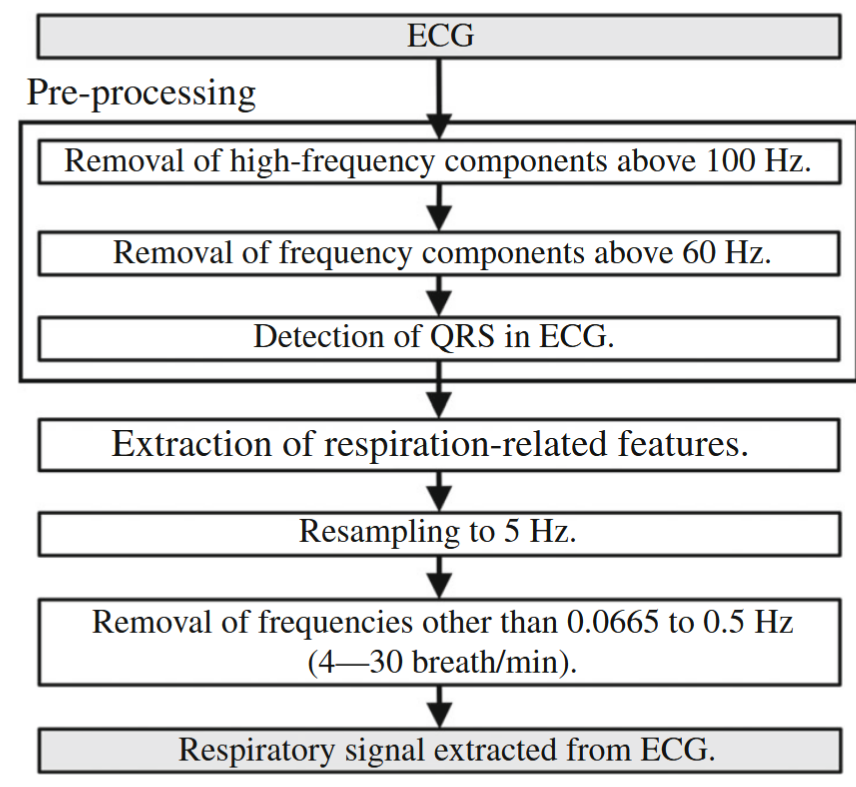
\includegraphics[width=6cm]{EDR_pipeline_akai}
            \caption{The typical pipeline for deriving respiratory signals from ECGs. Note that Akai et al. used signals with a frequency of 1000Hz, so exact values for pre-processing may differ from study to study. Diagram from \textcite{akaiReducingRespiratoryArtifacts2026}.}
            \label{EDRpipeline}
      \end{centering}
\end{figure}
\nl
The language used is python, and the code for calculating the EDR can be found in \ref{EDRconverter}. The numpy arrays for both the EDR and time were saved in the .npz format - a zipped archive format used to store numpy arrays. The code was able to convert and save the EDR and time at an average of about 6 seconds per record. The time taken is heavily dependent on the length of the record, which can range from 7 to 10 hours \cite{pollard_physionet_2026}.
\par
The obtained EDR is itself not a direct measure of the respiratory rate, but rather the respiratory effort. The breathing rate is estimated by performing a Short Time Fourier Transform (STFT) with a time window of 30 seconds. Then, the breathing rate over a 30-second period is the frequency with the highest peak in the spectrogram in that time period. \par
The database also provides additional respiratory measurements for select records, which include Chest and Abdominal respiratory effort signals obtained using respiratory inductance plethysmography (RIP), a technique which estimates changes in lung volume by non-invasively measuring contractions and expansions of the adbomen and thorax \cite{mehraChapter14Evaluation2009}. We use these measurements as validation for the EDR derivation method that we described above. \par
Plotting the spectrogram of the EDR can reveal visual patterns which could provide 'tells' for Apnoea. We will also use spectrograms to compare the EDR with experimental measurements of respiration efforts.

\section{Computer code}\label{sec:code}
\subsection{Code input/output}\label{subsec:codeinout}

\subsection{Code written verbatim}\label{subsec:verbatim}

This can be done with the \texttt{listings} and \texttt{verbatim} packages. You should modify the preamble document so that these packages correctly interpret the programming language that you used.
\nl
This will eventually be replaced with real code used for the project.

\begin{lstlisting}[label={EDRconverter}]
      def ...
\end{lstlisting}

\begin{lstlisting}
      FUNCTION PINEWT(N)
      IMPLICIT DOUBLE PRECISION (A-H,O-Z)
C**********************************************************************C
C     PINEWT EVALUATES THE INFINITE SERIES REPRESENTATION              C
C     FOR PI AS A TRUNCATED SUM.                                       C
C**********************************************************************C
C
C     ENSURE N IS A LEGAL VALUE
      IF(N.LT.0) THEN
        WRITE(6,*) 'In PINEWT: illegal value for N.',N
        RETURN
      ELSEIF(N.EQ.0) THEN
        PINEWT = 2.0D0
      ENDIF
C
C     INITIALISE SOME COUNTERS
      TWOPOW = 1.0D0
      FACKNM = 1.0D0
      FACKDM = 1.0D0
      PINEWT = TWOPOW*FACKNM*FACKNM/FACKDM
C
C     LOOP OVER SERIES ORDER N TIMES, ADDING EACH TERM TO TOTAL
      DO I=1,N
        TWOPOW = 2.0D0*TWOPOW
        FACKNM = DFLOAT(I)*FACKNM
        FACKDM = DFLOAT(2*I+1)*DFLOAT(2*I)*FACKDM
        PINEWT = PINEWT + TWOPOW*FACKNM*FACKNM/FACKDM
      ENDDO
C
C     DOUBLE THE RESULT (SEE WIKIPEDIA FORMULA)
      PINEWT = 2.0D0*PINEWT
C
      RETURN
      END
\end{lstlisting}